\chapter{Existing Approaches to Container Energy Consumption}
\label{chap:tool-analysis}

\section{Introduction}
\label{sec:tool-intro}

Accurately measuring and attributing energy consumption in containerized environments has become a central challenge in sustainable cloud computing. As container orchestration platforms like Kubernetes grow in adoption, the need for energy observability at finer granularities—down to the container or even process level—becomes increasingly critical. This requirement stems from a range of applications, including cost optimization, carbon accounting, energy-aware scheduling, and performance tuning.

A number of tools and frameworks have emerged in recent years to address this problem. Some focus on the system or server level, exposing power metrics via standardized interfaces or external instrumentation. Others adopt telemetry-based estimation approaches that infer energy usage from resource utilization statistics. More recently, several tools have begun to target container-level energy attribution specifically, often by integrating with Kubernetes and leveraging technologies such as eBPF, RAPL, and cgroups.

This chapter surveys the landscape of existing tools, organized into three categories: system-level monitoring solutions, telemetry-based estimation frameworks, and container-focused energy attribution tools. Particular attention is given to tools that support Kubernetes environments, as these are directly relevant to the goals of this thesis. Each tool is analyzed based on its architecture, metric sources, modeling approach, and practical limitations. Later sections discuss the emerging tool KubeWatt and present a comparative synthesis of strengths and weaknesses across the reviewed solutions.

\section{Non-container-focused Energy Monitoring Tools}
\label{sec:non-k8s-tools}
\subsection{Server-Level Energy Monitoring}
\label{sec:server-tools}
While not directly translatable to container-level energy monitoring, server-level energy consumption is an important aspect of it. Scientific works and tools in this domain generally don't provide the temporal resolution required for container-level energy monitoring.

\subsubsection{Kavanagh and Djemame: Energy Modeling via IPMI and RAPL Calibration}
\label{sec:kavanagh}

\paragraph{Overview and Architecture}
Kavanagh and Djemame\parencite{kavanagh2019rapid} present their findings on combining IPMI and RAPL (interface unspecified) data to estimate server energy consumption, achieving improved accuracy through calibration with an external server-level Watt meter. For calibration, they induce artificial CPU workloads and rely on CPU utilization metrics with 1-minute averaging windows, necessitating extended calibration intervals to obtain stable readings. While the resulting model is tailored to their specific hardware and not generally portable, their work provides valuable insights into the complementary use of IPMI and RAPL. The authors recognize that the respective limitations of these tools (RAPL’s partial scope and IPMI’s low resolution) can be mitigated when used in combination.

\paragraph{Attribution Method and Scope}
Although the model operates at the physical host level, it supports attribution to VMs or applications using CPU-utilization-based proportional allocation. Several allocation rules are proposed, including utilization ratio, adjusted idle sharing, and equal distribution. However, no container-level attribution is attempted, and runtime flexibility is limited due to the static nature of the calibration.

\paragraph{Validation and Limitations}
With their Watt-meter-calibrated model using segmented linear regression, the authors report an average error of just -0.17\%. More relevant to practical application, they also construct a model based solely on IPMI and RAPL(calibrated via Watt meter data) which achieves a reduced error of -5.58\%, compared to -15.75\% without calibration. Limitations of their approach include the need for controlled, synthetic workloads, coarse-grained sensor input, and the assumption of relatively stable system conditions during calibration.

\paragraph{Key Contributions}
\begin{itemize}
    \item \textbf{Hybrid use of IPMI and RAPL is analyzed}, showing that these tools compensate for each other’s limitations. RAPL underestimates total system power, while IPMI captures more components but at lower resolution.
    \item IPMI accuracy is significantly improved through external Watt meter calibration.
    \item The authors provide practical calibration guidelines:
    \begin{itemize}
        \item Use long, static workload plateaus to align with averaging windows and reduce synchronization complexity.
        \item Discard initial and final measurement intervals to avoid transient noise and averaging artifacts.
        \item Ensure calibration workloads exceed the IPMI averaging window to capture valid steady-state values.
    \end{itemize}
\end{itemize}

\paragraph{Relevance to Proposed Architecture}
This work informs the proposed architecture by demonstrating how combining RAPL and IPMI can yield more accurate system-level power estimation. The use of plateau-based calibration and composite data models is especially applicable. However, the lack of container-level granularity, reliance on offline calibration, and limited attribution scope underscore the need for more dynamic, fine-grained, and container-aware approaches in Kubernetes-based environments.

\subsubsection{CodeCarbon}
CodeCarbon\parencite{codecarbon_2024} is a Python package designed to estimate the carbon emissions of a program’s execution. While its implementation is general-purpose, it is primarily aimed at machine learning workloads.

\paragraph{Overview and Architecture}
CodeCarbon estimates a workload’s energy consumption by relying on RAPL \textit{package-domain} CPU metrics via the \code{powercap} RAPL file system interface. A fix for the RAPL MSR overflow issue was implemented\parencite{codecarbon_issue_322}. In the absence of RAPL support, it falls back to a simplified model based on the CPU’s Thermal Design Power (TDP), obtained from an internal database, and combines it with CPU load metrics from \code{psutil}. For memory, a static power value is assumed based on the number and capacity of installed DIMMs. GPU power consumption is estimated via NVIDIA’s NVML interface. The default measurement interval is 15 seconds, with the authors citing lightweight design as the primary motivation.

The component-level estimations are then aggregated and multiplied by a region-specific net carbon intensity (based on the local electricity grid’s energy mix) to estimate the program’s total CO\textsubscript{2} emissions. CodeCarbon is typically executed as a wrapper around code blocks, scripts, or Python processes.

\paragraph{Limitations}
There is no direct attribution of CPU activity to individual power metrics: CodeCarbon estimates energy use indirectly, based on the number of active cores and average CPU utilization, while making many assumptions that could be prevented. Combined with the relatively long measurement intervals, this results in background system processes also being attributed to the measured Python program. Consequently, CodeCarbon does not contribute directly to the goals of this thesis, which seeks fine-grained, container-level attribution.

However, the tool highlights several interesting secondary considerations. The integration of regional CO\textsubscript{2} intensity data is a valuable extension to conventional energy measurement and is well implemented. Additionally, the Python-based design offers high accessibility and ease of use, which may serve as inspiration for future developer-facing tools.

\subsubsection{AI Power Meter}
\textit{AI Power Meter}\parencite{aipowermeter} is a lightweight Python-based tool designed to monitor the energy consumption of machine learning workloads. It gathers power consumption data for the CPU and RAM via Intel RAPL using the \code{powercap} interface, and for the GPU via NVIDIA’s NVML library. While the authors acknowledge that other system components (e.g., storage, network) also contribute to energy usage, these are not currently included and are considered an accepted limitation of the tool.

Unlike more advanced attribution tools, AI Power Meter does not distinguish between individual processes or workloads. Instead, it provides coarse-grained, system-level energy consumption measurements over time. In this respect, its scope is similar to \textit{CodeCarbon}, focusing on ease of use and integration into ML pipelines rather than precise, per-process energy attribution. As such, while not directly applicable to container-level measurement or power attribution, AI Power Meter demonstrates the growing interest in accessible energy monitoring tools within the machine learning community.

\subsection{Telemetry-Based Estimation Frameworks}
\label{sec:telemetry-tools}

\subsubsection{PowerAPI Ecosystem\parencite{powerapi2024github} (PowerAPI, HWPC, SmartWatts)}
\label{sec:powerApiFramework}

PowerAPI\parencite{fieni2024powerapi} is an open-source middleware toolkit for assembling software-defined power meters that estimate real-time power consumption of software workloads. Developed as a generalized and modular framework, PowerAPI evolved alongside specific implementations such as \textit{SmartWatts}, detailed in section~\ref{sec:smartwatts}. It allows power attribution at multiple granularity levels, including processes, threads, containers, and virtual machines. A distinctive strength of PowerAPI is the continuous self-calibration of its power models, enabling accurate real-time energy estimation under varying workloads and execution conditions. This makes PowerAPI particularly suited to heterogeneous computing infrastructures.

\paragraph{Overview and Architecture}

PowerAPI uses an actor-based model for modularity, enabling easy customization of its internal components with minimal coupling. It supports raw metric acquisition from diverse sensors (e.g., physical meters, processor interfaces, hardware counters, OS counters) and delivers power consumption data through various output channels (including files, network sockets, web interfaces, and visualization tools). As middleware, PowerAPI facilitates assembling power meters "\textit{à la carte}" to accommodate specific user requirements and deployment scenarios.

\paragraph{Core Components}
\begin{itemize}
    \item \textbf{powerapi-core}: Middleware orchestrating real-time/post-mortem interactions between sensors and formulas. It defines the essential interfaces for sensor data ingestion and output channels (e.g., MongoDB, InfluxDB, CSV, socket, Prometheus), and includes built-in capabilities for data preprocessing, postprocessing, and reporting.
    \item \textbf{hwpc-sensor}: A telemetry probe designed to gather low-level hardware performance counters (HWPCs), including instructions, cycles, and RAPL energy metrics. This sensor leverages \textit{perf} and \textit{cgroups-v2}, critical for fine-grained telemetry in containerized environments. It also provides detailed CPU performance state metrics via MSR events (\code{TSC}, \code{APERF}, \code{MPERF}).
    \item \textbf{SmartWatts-formula}\parencite{fieni2020smartwatts}: A power model implementation (in Python) using HWPC data to estimate power consumption dynamically. It employs online linear regression provided by the Python \textit{scikit-learn}\parencite{scikit-learn} library, enabling accurate runtime learning of workload-specific power signatures. SmartWatts is further detailed in section~\ref{sec:smartwatts}.
    \item \textbf{SelfWatts-controller}: Dynamically selects hardware performance counters for software-defined power models, facilitating automatic configuration and unsupervised deployment in heterogeneous infrastructures. Currently, its development has stalled for several years, limiting its practical applicability.
    \item \textbf{pyRAPL}: A convenient Python wrapper around RAPL for CPU, DRAM, and iGPU energy metrics collection, providing easy access to hardware-based power data.
\end{itemize}

\paragraph{Relevance and Integration}
The modular and extensible architecture of PowerAPI positions it as a highly suitable foundation for further research and development of specialized power attribution tools. Researchers can readily extend or adapt its components to address evolving or niche requirements. However, its current implementation does not incorporate certain critical metrics, such as IPMI-based telemetry, which could limit its completeness in some practical deployment scenarios. Nonetheless, PowerAPI represents a significant advancement toward the creation of generalized, plug-and-play power models that operate without extensive manual calibration. This emphasis on practical deployability and general applicability highlights a key strength of the project and sets a clear direction for future research and development efforts in the domain of software-defined energy monitoring.

\subsubsection{Green Metrics Tool}

The \textit{Green Metrics Tool} (GMT)\parencite{greencodingdocs} is an open-source framework designed to measure the energy consumption of containerized applications across various phases of the software lifecycle, including installation, boot, runtime, idle, and removal. It uses small, modular metric collectors to gather host-level energy and system data (e.g., CPU and DRAM energy via RAPL, IPMI power readings), and is orchestrated through declarative usage scenarios.

While GMT provides reproducible, lifecycle-aware measurements in controlled environments, it does \textit{not} perform container-level or process-level energy attribution. The developers explicitly avoid splitting energy consumption across containers, citing the lack of reliable attribution models.

\section{Container-Focused Energy Attribution Tools}
\label{sec:container-tools}

While system-level monitoring and telemetry-based estimation provide valuable insights into overall server energy consumption, they fall short when it comes to attributing energy use to individual containers. In multi-tenant or microservice-based environments, such granularity is essential for accurate accountability, optimization, and scheduling decisions. 

This section focuses on tools specifically designed to address this challenge by providing energy attribution at the level of containers or processes within a containerized environment. These tools typically integrate with container runtimes and Kubernetes, leveraging sources such as hardware counters, control groups, and performance monitoring frameworks to estimate or infer energy consumption.

The following subsections analyze three prominent tools (Kepler, Scaphandre, and SmartWatts) each with a distinct architectural approach. A fourth tool, KubeWatt, is discussed separately as a derivative implementation developed in response to identified limitations in Kepler.

\subsection{Kepler}
\label{sec:kepler}

\subsubsection{Overview and Goals}
\label{sec:kepler-overview}

Kepler (\textit{Kubernetes-based Efficient Power Level Exporter})\parencite{kepler_energy} is a modular, Kubernetes-native framework for monitoring, modeling, and estimating energy consumption in containerized environments. As the most prominent tool for container-level power estimation in Kubernetes, Kepler enables detailed observability of energy usage at the level of individual processes, containers, pods, and nodes\parencite{amaralKeplerFrameworkCalculate2023}.

Kepler integrates seamlessly with Kubernetes and Prometheus-based observability stacks. It supports both real-time energy metrics (e.g., RAPL, ACPI, NVML) and model-based estimation through trained regression models, making it applicable across a wide range of deployment environments, from bare-metal servers to virtual machines. Developed as an open-source CNCF project, Kepler’s architecture is designed to be extensible, allowing researchers and practitioners to contribute new power models and adapt it to diverse system architectures.

It should be noted that shortly before the completion of this thesis, version 0.10.0 of Kepler was released. This version constitutes a major architectural rewrite of the project, intended to address structural limitations of earlier versions. However, the analysis in this chapter focuses on Kepler versions 0.9.x and earlier, which remain the most widely deployed at the time of writing. Section~\ref{sec:kepler-new-version} briefly summarizes the key changes introduced in the new release.
\subsubsection{Architecture and Metric Sources}
\label{sec:kepler-architecture}

Kepler's architecture consists of several interconnected components, with the core functionality centered around a privileged monitoring agent that runs on every node. While the framework supports model-based estimation for environments without hardware telemetry, this thesis focuses on the direct collection of real-time power and utilization metrics available in bare-metal deployments.

\paragraph{Deployment Models}
Kepler supports multiple deployment scenarios depending on the availability of energy sensors on the host system. In bare-metal environments, Kepler can directly collect power metrics using RAPL, ACPI, or Redfish/IPMI interfaces. This is the most accurate and relevant mode for the purpose of this thesis. In contrast, on virtual machines (VMs), where access to hardware counters or power interfaces is restricted, Kepler relies on trained regression models to estimate node-level energy consumption. A third, currently unimplemented deployment model proposes a passthrough mechanism where a host-level Kepler instance would expose power metrics to a nested Kepler instance inside the VM. These deployment models are visualized in figure~\ref{fig:kepler-deployment-modes}.

\begin{figure}[ht]
  \centering
  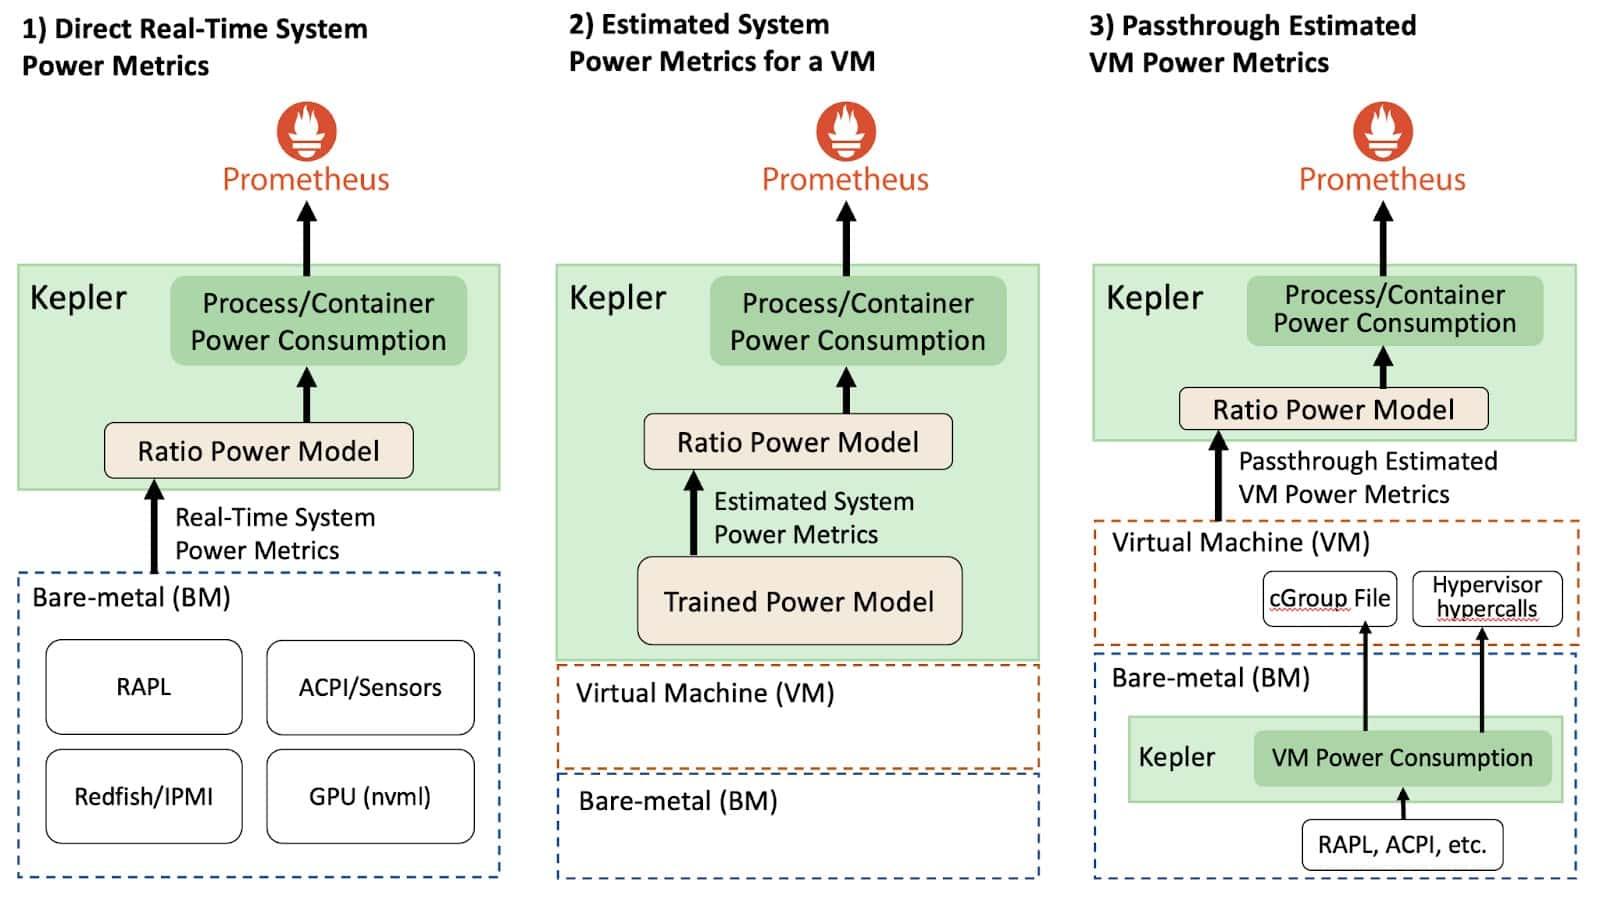
\includegraphics[width=0.8\textwidth]{Figures/kepler_deployment_modes.jpg}
  \caption{Kepler deployment models: direct power measurement on bare-metal, estimation on VMs, and the proposed passthrough model (currently not implemented)\parencite{kepler_docs}}
  \label{fig:kepler-deployment-modes}
\end{figure}

\paragraph{Kepler Agent and Exporter}
The core monitoring functionality is handled by the Kepler Agent, which is deployed as a privileged DaemonSet pod on each Kubernetes node. It collects energy and resource utilization metrics using a combination of eBPF instrumentation and hardware performance counters exposed via \code{perf\_event\_open}. A kprobe attached to the \code{finish\_task\_switch} kernel function enables accurate tracking of per-process context-switch activity. Container and pod attribution is performed after parsing the cgroup path from \path{/proc/<pid>/cgroup} and querying the Kubelet API for container metadata. The generated metrics are exported via a Prometheus-compatible endpoint for downstream processing and visualization. A generalized information flow is shon in figure~\ref{fig:kepler-architecture}.

\begin{figure}[ht]
  \centering
  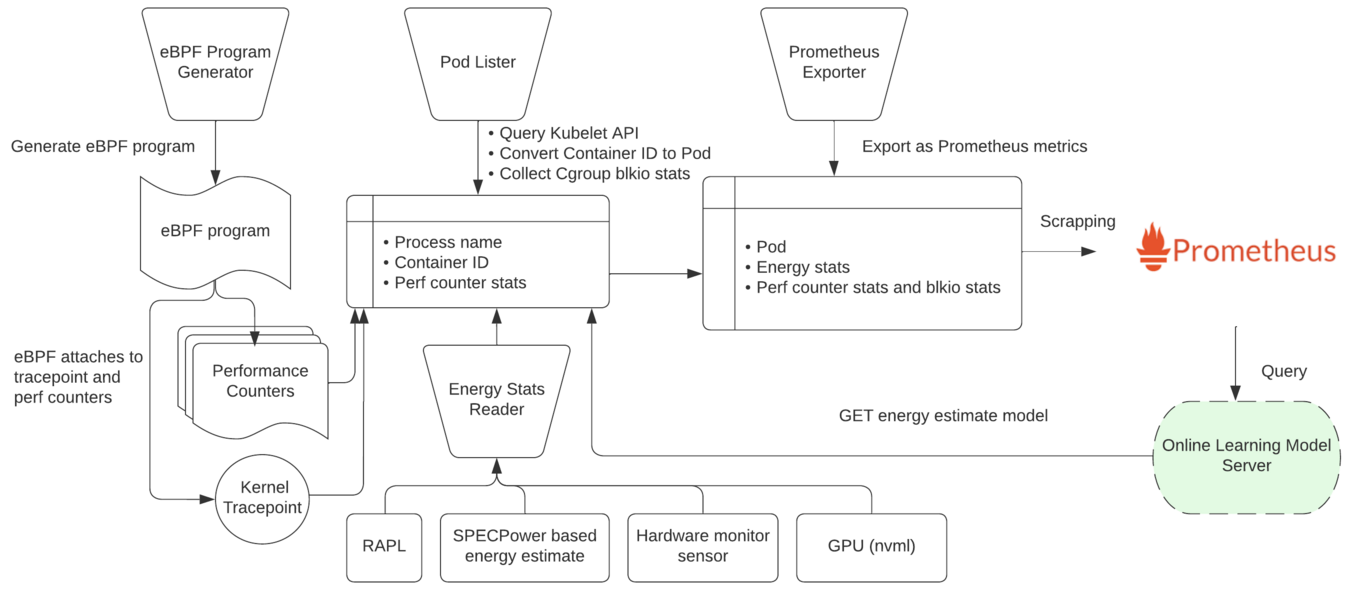
\includegraphics[width=0.9\textwidth]{Figures/kepler_architecture.png}
  \caption{Simplified architecture of the Kepler monitoring agent and exporter components\parencite{kepler_docs}}
  \label{fig:kepler-architecture}
\end{figure}


\paragraph{Resouce Utilization via eBPF-based Hardware/Software Counters}

To measure low-level CPU activity, Kepler uses the Linux syscall \code{perf\_event\_open} to configure hardware performance counters on each core. The following events are tracked:
\begin{itemize}
  \item \code{PERF\_COUNT\_HW\_CPU\_CYCLES}: Total CPU cycles (affected by DVFS)
  \item \code{PERF\_COUNT\_HW\_REF\_CPU\_CYCLES}: Frequency-independent cycles
  \item \code{PERF\_COUNT\_HW\_INSTRUCTIONS}: Retired instructions
  \item \code{PERF\_COUNT\_HW\_CACHE\_MISSES}: Last-level cache misses
\end{itemize}

These counters are accessed via BPF perf event arrays. On each context switch, current counter values are sampled, and deltas are computed against previously stored values. These deltas represent the CPU activity of the process leaving the CPU and are stored in BPF maps for later aggregation.

In addition to hardware counters, Kepler collects several software-level metrics that are not natively exposed by the Linux kernel. These include CPU time, page cache activity, and interrupt handling statistics. Because these metrics are unavailable through standard interfaces, Kepler uses custom eBPF programs to infer them from kernel behavior.

Since version~0.7, Kepler has migrated to \code{libbpf} and uses a BTF-enabled kprobe to instrument the \code{sched\_switch} function. This allows Kepler to safely extract process IDs and timing data without relying on fragile symbol offsets. On each context switch, Kepler records timestamps and uses them to increment the \code{CPUTime} counter, providing fine-grained accounting of CPU residency per process.

Other software counters include:
\begin{itemize}
  \item \code{PageCacheHit}: Tracks read and write access to the page cache using eBPF programs attached to \code{mark\_page\_accessed} and \code{writeback\_dirty\_folio}.
  \item \code{IRQNetTX}, \code{IRQNetRX}, \code{IRQBlock}: Count the number of softirq events attributed to a process, using the \code{softirq\_entry} tracepoint.
\end{itemize}

Each of these metrics is manually accumulated in eBPF maps keyed by process ID and periodically read by the user-space collector. This enhances energy attribution, especially in scenarios where hardware counters are insufficient or unavailable.

\paragraph{Node Component-level energy consumption via RAPL}
Kepler supports component-level power estimation by reading RAPL energy counters, focusing on the \code{core}, \code{uncore}, \code{package}, and \code{dram} domains. The energy values are read via the \code{PowerCap} Framework using the \path{/sys/class/powercap} interface. The sysfs path tree is parsed dynamically to detect available domains and sockets, ensuring compatibility across architectures and CPU generations. Energy values are read directly from files such as \code{energy\_uj} and divided by 1000 to yield millijoule-level readings. A wraparound detection mechanism ensures robustness even when energy counters overflow.

The core logic is implemented in \code{UpdateProcessEnergy()}, which is invoked periodically by the main metrics collection loop (and also calls the process attribution logic immediately after the metrics update). However, despite RAPL's native ability to provide energy readings at approximately millisecond-level resolution, Kepler limits energy sampling to a coarse default interval of three seconds (defined in \code{config.SamplePeriodSec}). This choice reflects a trade-off between performance overhead and metric granularity, but may limit the accuracy for short-lived or bursty workloads.

Importantly, Kepler does not rely on eBPF or perf events to retrieve energy values; energy is obtained entirely through file-based reads from sysfs or, on some platforms, via MSR or hwmon fallbacks. The collected energy values are later exposed to Prometheus and used in model training and runtime inference. The measurement cadence, attribution methodology, and available domains are validated using an internal tool that checks domain availability and collects average power readings across repeated samples.

\paragraph{Platform-Level Energy Consumption}
Kepler supports platform-level energy monitoring through external power interfaces exposed by the underlying server hardware. These measurements represent the total energy consumed by the entire node, as opposed to specific hardware components or processes. The implementation is modular, with each power source encapsulated in a corresponding \code{source} module. Currently supported backends include ACPI (via the \path{/sys/class/hwmon} interface), Redfish (via the Redfish REST API), and a stub for IBM's HMC interface on \code{s390x} systems.

Among these, Redfish provides the most detailed and reliable node-level power data. It queries the server's BMC for the \code{PowerConsumedWatts} value using a REST endpoint. This value is then converted into energy (in milliJoules) by multiplying with the time elapsed since the previous query. Kepler spawns a background goroutine that polls this value at regular intervals (user-configurable via the \code{REDFISH\_PROBE\_INTERVAL\_IN\_SECONDS} parameter in the Kepler configuration). This design allows Redfish to provide cumulative energy measurements with known sampling resolution.

ACPI-based sources offer an alternative when Redfish is unavailable. These rely on instantaneous power averages and do not necessarily represent total node power. The HMC source, by contrast, is currently a non-functional placeholder used only on unsupported platforms. Overall, platform-level metrics are treated as node-wide aggregate energy values without internal attribution, but they offer valuable ground truth for cross-validating other metrics or monitoring infrastructure-level power trends.

\paragraph{Metadata Inputs for Container, System, and VM Attribution}

To organize energy and resource metrics by container, Kepler collects metadata that maps processes to Kubernetes pods, containers, and namespaces. Kepler supports both cgroups v1 and v2 and dynamically traverses \code{/sys/fs/cgroup} to map \code{PID} or \code{cgroupID} values to container IDs, extracting the last 64 characters of valid cgroup paths.

If the container ID is not cached, Kepler queries Kubernetes for pod metadata using either the Kubelet's local \code{/pods} API or, if enabled, the Kubernetes API server via a dedicated watcher. Both approaches extract metadata from \code{ContainerStatuses} fields in pod objects and populate a shared cache. This includes support for init and ephemeral containers. Container ID prefixes are stripped using regex to standardize the format.

Processes not associated with a container are labeled using fallback logic. If the process belongs to the root cgroup (\code{cgroupID = 1}) and cgroup-based resolution is enabled, it is labeled \code{container="kernel\_processes"}, \code{namespace="kernel"}. All other unmapped processes are labeled \code{container="system\_processes"}, \code{namespace="system"}. This includes host services such as \code{kubelet}, \code{containerd}. The Linux idle thread (PID 0), which does not appear in \code{/proc} and cannot be queried like regular processes, is not explicitly handled by Kepler; however, since it belongs to the root cgroup implicitly, it is effectively included under the \code{kernel\_processes} label.

In addition to container and system process tracking, Kepler supports experimental attribution for virtual machines running under QEMU/KVM on the host. When executed on the hypervisor, Kepler scans \code{/proc/<pid>/cgroup} for scope names matching the systemd pattern \code{machine-qemu-*.scope} to identify VM processes. If a match is found, the VM ID is extracted and used to create a \code{VMStats} structure, allowing the VM to be tracked similarly to a container. Optionally, a metadata lookup via the libvirt API can be used to resolve human-readable VM identifiers. This enables Kepler to expose VM-level resource and energy metrics on systems that mix containers and virtual machines. However, this mechanism only applies to Kepler instances running on the VM host and does not provide visibility into containers running inside the VM.

This metadata layer allows Kepler to cleanly separate containerized workloads, system processes, kernel activity, and virtual machines, ensuring complete coverage of energy attribution in subsequent stages.

\paragraph{GPU Power- and Resource Utilization via NVML}

Kepler collects per-process GPU utilization statistics using the NVIDIA Management Library, accessed through internal Go bindings. Specifically, Kepler queries both compute engine usage and memory utilization for each process interacting with an NVIDIA GPU. This data is retrieved via the \code{ProcessResourceUtilizationPerDevice()} method, which internally calls NVML functions like \code{nvmlDevice.GetProcessUtilization} to return process statistics, including Streaming Multiprocessor utilization (\code{SmUtil}), memory utilization (\code{MemUtil}), and optional encoding/decoding activity. Additionally, KEPLER collects GPU energy consumption using NVML's \code{getPowerUsage}.

To support NVIDIA's Multi-Instance GPU (MIG) architecture, Kepler first inspects whether MIG slices exist on a given device. If so, it iterates over each slice and retrieves+ per-process utilization data individually. Otherwise, it queries the full physical GPU. In both cases, the parent GPU ID is used as the key to unify resource attribution. For each PID returned by NVML, GPU utilization metrics are appended to the \code{ResourceUsage} field of the Kepler-internal \code{ProcessStats} structure. The following metrics are collected:
\begin{itemize}
  \item \code{GPUComputeUtilization}: The percentage of compute engine usage (SM activity) over the sampling interval.
  \item \code{GPUMemUtilization}: The percentage of frame buffer memory usage per process.
\end{itemize}

Because NVML does not provide high-resolution energy counters, Kepler approximates GPU energy consumption by multiplying the instantaneous device-level power draw (\code{GetPowerUsage}) with the sampling interval duration (\code{SamplePeriodSec}). That is, energy per device is estimated as \code{energy=power(mW)$\times$SamplePeriodSec}. This coarse-grained sampling, typically performed every few seconds, limits the temporal resolution and may miss short-lived GPU activity.

If \code{GetProcessUtilization()} is not supported by the hardware or fails at runtime, Kepler falls back to using \code{GetComputeRunningProcesses()} combined with per-process memory usage to estimate GPU utilization. In this mode, energy is attributed proportionally to memory usage rather than compute activity. Alternative backends such as Habana or DCGM are supported but do not offer per-process utilization data, and are thus not used for fine-grained attribution in Kepler’s default configuration.

\paragraph{Summary if Inputs}
Tables~\ref{tab:kepler-metric-inputs} and~\ref{tab:kepler-metadata-inputs} summarize the distinct types of input Kepler collects. Metric inputs provide raw resource and energy data, while metadata inputs allow this data to be mapped to containers, VMs, or system processes.

\begin{table}[h]
    \small
    \centering
    \begin{tabular}{ |L{4.5cm} | L{5cm} | L{4.5cm}| } 
        \hline
        \textbf{Metric Type} & \textbf{Source} & \textbf{Purpose} \\
        \Xhline{1.5pt}
        CPU hardware counters & \code{perf\_event\_open} via eBPF & Track cycles, instructions, cache misses per process \\
        \hline
        CPU software counters & Custom eBPF programs & Capture CPU time, IRQs, page cache activity \\
        \hline
        RAPL energy counters & \code{/sys/class/powercap} & Direct energy measurement for CPU and memory domains \\
        \hline
        Platform power & Redfish REST API, ACPI sysfs & Estimate total node energy from external sensors \\
        \hline
        GPU utilization & NVML (via Go bindings) & Track per-process compute and memory usage \\
        \hline
        GPU energy (approx.) & NVML power reading $\times$ interval & Estimate per-device energy usage \\
        \hline
    \end{tabular}
    \caption[Metric inputs used by Kepler]{Metric inputs used by Kepler for energy and resource monitoring}
    \label{tab:kepler-metric-inputs}
\end{table}

\begin{table}[h]
    \small
    \centering
    \begin{tabular}{ |L{4.5cm} | L{5cm} | L{4.5cm}| } 
        \hline
        \textbf{Metadata Type} & \textbf{Source} & \textbf{Purpose} \\
        \Xhline{1.5pt}
        Container ID extraction & \code{/proc/<pid>/cgroup} & Identify container context of each process \\
        \hline
        Pod and namespace info & Kubelet API or Kubernetes API server & Map container ID to pod, namespace, container name \\
        \hline
        System process fallback & Internal constants + missing container ID & Label processes outside containers as \code{system\_processes} \\
        \hline
        Kernel thread fallback & \code{cgroupID = 1} & Label root-cgroup processes as \code{kernel\_processes} \\
        \hline
        Virtual machine ID & \code{machine-qemu-*.scope} + optional libvirt lookup & Label QEMU/KVM-based VMs by scope or libvirt metadata \\
        \hline
        GPU process association & PID-based matching via NVML & Associate GPU usage with Linux processes \\
        \hline
    \end{tabular}
    \caption[Metadata inputs used by Kepler]{Metadata inputs used by Kepler to organize and label monitored workloads}
    \label{tab:kepler-metadata-inputs}
\end{table}

\paragraph{Export Interface and Metric Exposure}

All metrics collected by Kepler are ultimately exposed via Prometheus after power attribtion. This includes both raw utilization metrics (e.g. CPU time, instructions, cache misses) and derived energy metrics (e.g. power estimates per container). The Prometheus export format allows flexible time series queries and integration with Grafana or other observability platforms.

\paragraph{Estimator Sidecar and Model Inference}

In addition to its lightweight internal estimator, Kepler optionally supports an estimator sidecar container that uses more sophisticated regression models for power inference. The sidecar communicates with the exporter via a Unix domain socket and loads pre-trained models (e.g. Scikit-learn, XGBoost) suitable for online estimation in environments lacking direct power metrics. This mechanism is mainly intended for telemetry-sparse environments and is not used in the real-time deployment mode considered in this thesis.

\paragraph{Model Server and Model Training}

For environments where energy measurement is available (e.g. via RAPL or Redfish), Kepler provides a separate model server that facilitates training of machine learning-based energy models. This component ingests time-aligned Prometheus metrics and energy readings, applies preprocessing steps, and generates regression models that estimate power consumption based on utilization metrics. Both absolute and dynamic models can be trained, using different feature groups (e.g., time-based vs instruction-based) and labeled according to power domain (e.g. core, package). The resulting models are stored in a hierarchical directory format and can be deployed in other environments via the estimator sidecar. The model server supports modular pipelines, allowing flexible input data sources, energy isolation techniques, and regression backends. This training loop is essential in contexts where hardware telemetry is available during development or profiling but not in production. While model training plays a key role in extending Kepler to new environments\parencite{choochotkaewAdvancingCloudSustainability2023}, it is not central to the goals of this thesis.

\paragraph{External Integration}

Kepler is designed to integrate seamlessly with existing observability tools. Prometheus is used to scrape metrics from the Kepler agent, and dashboards can be built using Grafana to visualize energy consumption across nodes, containers, or applications. While not required for the core functionality, this integration facilitates operational awareness and debugging.

\subsubsection{Attribution Model and Output}
\label{sec:kepler-attribution}

\paragraph{Kepler Configurability and Measurement Interval}
Kepler updates its input metrics at a configurable interval (default: \texttt{SamplePeriodSec} = 3 seconds), with the exception of Redfish-based measurements, which have a separate, user-defined interval (default: 15 seconds). Although utilization and RAPL energy metrics theoretically support more fine-grained sampling, Kepler performs attribution based solely on aggregated values within each configured sampling window. While this reduces system overhead, it may miss short-lived energy fluctuations. Kepler's attribution framework is modular by design, allowing for easy integration of new power sources through standardized interfaces. Depending on the availability of input metrics, Kepler uses either direct power readings or model-based estimation. In the absence of hardware telemetry (i.e. RAPL), Kepler can apply regression models trained on a reference system where accurate power readings are available. For this thesis, only scenarios where all relevant metrics are available (as discussed in Chapter~\ref{sec:kepler-architecture}) are considered.

\paragraph{Division of Power into Idle and Dynamic Components}
Kepler conceptually divides total power consumption into \emph{idle power} and \emph{dynamic power}. Their sum constitutes the total (often named \emph{absolute} power) measured energy on both process and node levels. Dynamic power is correlated with resource utilization, while idle power represents the static baseline consumption that persists regardless of system activity. This distinction is critical, as Kepler distributes these two components differently among processes~\parencite{amaral2023exploring}. Idle power attribution follows the Greenhouse Gas Protocol guidelines~\parencite{gesi2024ictguidance}, which recommend splitting idle power across containers based on their size (i.e. resource requests relative to the total). Dynamic power, by contrast, is attributed proportionally to observed resource usage.

\paragraph{Node-Level Energy Attribution}
On the node level, Kepler directly uses RAPL energy readings from the \texttt{pkg}, \texttt{core}, \texttt{uncore}, and \texttt{dram} domains for all available sockets, reporting energy in millijoules. GPU energy is measured per device via NVML. Platform-level energy is retrieved via the configured source, typically Redfish. Kepler iterates through all exposed chassis members and internally converts Redfish power metrics (in watts) to milliwatts, which are then multiplied by \texttt{SamplePeriodSec} to produce energy values in millijoules. These can then be treated like standard metrics.\\
After collecting node-level energy metrics, Kepler updates the tracked \emph{minimum idle power} if a new lower value is observed. The corresponding resource usage is also recorded. This tracking applies to all RAPL domains and GPU devices. Node-level dynamic energy is computed as the difference between total and idle energy. Additionally, Kepler calculates the residual category \emph{Other} as platform power minus the sum of \texttt{pkg}, \texttt{dram}, and GPU power, separately for idle and dynamic metrics. This implicitly attributes all remaining energy to unspecified components (e.g. network interfaces, fans, or storage devices).

\paragraph{Process-Level Energy Attribution}
Process energy is attributed based on resource utilization metrics and node-level energy values. Using the most recent measurements of component, GPU (if enabled), and platform power, Kepler calculates each process’s energy consumption.  
Idle energy is simply divided evenly among all processes. This is in contrast to Kepler’s documentation, which states that idle energy should be divided by requested container size (in accordance with the GHG protocol~\parencite{gesi2024ictguidance}). Since container-level metadata is aggregated from per-process statistics, implementing size-based idle attribution at the process level is non-trivial. Nonetheless, this feature is advertised but not implemented, as noted by a \texttt{TODO} comment in the codebase.

Dynamic energy is attributed proportionally using the formula:
\begin{equation}
E_{process_{dyn}} = \left\lceil E_{component_{dyn}} \cdot \frac{U_{process}}{U_{node}} \right\rceil
\end{equation}
where $U_{\text{process}}$ is the process's resource usage, and $U_{\text{node}}$ is the total component resource usage indicated by RAPL. If no usage is recorded, energy is divided evenly among processes. The specific usage metrics used in the default ratio model are:
\begin{itemize}
  \item \textbf{CPU}: based on \texttt{CPUInstructions} (fallback: \texttt{CPUTime})
  \item \textbf{DRAM}: based on \texttt{CacheMisses} (fallback: \texttt{CPUTime})
  \item \textbf{GPU}: based on \texttt{GPUComputeUtilization} (via NVML)
  \item \textbf{Other} and \textbf{Platform}: intended to use a configurable default metric
\end{itemize}
However, the default usage metric for \texttt{Uncore} and \texttt{Platform} domains is not set in the configuration, defaulting to an empty string. As a result, these metrics are not attributed based on usage and fall back to equal distribution. It is unclear whether this is a conscious design decision or an oversight.

The following formula~\ref{for:kepler_process_all} summarizes the complete energy attribution model used by Kepler at the process level. It combines all relevant energy domains: dynamic and idle energy across measured components (e.g. package, core, DRAM, uncore, GPU), as well as residual platform energy not accounted for by specific components. Each part of the equation reflects a distinct step in the attribution logic previously discussed, merging them into a single expression for total per-process energy consumption.

\begin{align}
    \label{for:kepler_process_all}
    E_{\text{process}} = \; &
    \sum_{\text{comp} \in \{\text{core}, \text{dram}, \text{uncore}, \text{gpu}\}} 
    \left(
    \left\lceil 
    E_{\text{comp}}^{\text{dyn}} \cdot \frac{U_{\text{process, comp}}}{U_{\text{node, comp}}} 
    \right\rceil
    + 
    \left\lceil 
    \frac{E_{\text{comp}}^{\text{idle}}}{N_{\text{processes}}} 
    \right\rceil
    \right) \notag \\
    & + 
    \left\lceil 
    \frac{E_{\text{platform}}^{\text{dyn}}  - \left(E_{\text{pkg}}^{\text{dyn}}  + E_{\text{dram}}^{\text{dyn}} \right)}{N_{\text{processes}}} 
    \right\rceil
    + 
    \left\lceil 
    \frac{E_{\text{platform}}^{\text{idle}}  - \left(E_{\text{pkg}}^{\text{idle}}  + E_{\text{dram}}^{\text{idle}} \right)}{N_{\text{processes}}} 
    \right\rceil
\end{align}

\subsubsection{Attribution Timing and Export Granularity}
\label{sec:kepler-attribution-timing}

Kepler attributes energy at fixed internal intervals (default: 3 seconds). These deltas are exposed via Prometheus metrics such as \texttt{kepler\_container\_joules\_total}, but the Prometheus scrape interval is user-defined and may not align with Kepler's update loop. If the export interval is not a multiple of the intermismatchesnal interval (e.g., 5s vs. 3s), metric misalignment can occur, leading to visible fluctuations even for stable workloads. Since Kepler does not smooth or interpolate values, this behavior is expected and intentional. For more stable time series, it is recommended to configure the export interval as a multiple of Kepler’s internal interval.

This timing issue primarily affects metrics that are reported as cumulative deltas (e.g. energy in millijoules). For Redfish-based metrics, which are provided in watts and converted internally by Kepler into energy values by multiplying with the update interval, synchronization is less problematic. The conversion to energy is performed over a well-defined window, which inherently matches the Prometheus export interval, thus avoiding the same class of timing.

\subsubsection{Validation and Research Context}

Kepler has been adopted in various academic and industrial settings as a tool for estimating energy consumption at the container and pod level. In most cases, it is treated as a black-box exporter, with little investigation into the reliability or internal consistency of its reported metrics. While its integration with Kubernetes and Prometheus makes it convenient to use, its internal attribution mechanisms and modeling assumptions are rarely scrutinized in published work. Andringa\parencite{andringa2024estimating} intestigates Kepler, but lacks the necessary depth.

A notable exception is the study by Pijnacker et al.~\parencite{pijnackerEstimatingContainerlevelPower2024,pijnackerContainerlevelEnergyObservability2025}, which constitutes the first dedicated empirical evaluation of Kepler’s behavior and attribution accuracy. Their work critically examines whether Kepler’s per-container energy metrics correspond to expected utilization and measured system-level power under controlled conditions.

To this end, the authors design a testbed using a Dell PowerEdge R640 with dual Intel Xeon CPUs, operating a single-node Kubernetes cluster. Redfish/iDRAC power readings, validated using a wall power plug, are used as a high-confidence ground truth reference. Container CPU metrics and metadata are collected using Prometheus and cAdvisor. Kepler is deployed in version 0.7.2, configured to use RAPL for component-level power metrics and Redfish for platform-level readings.

The validation experiment employs a repeated CPU stress workload (\code{stress-ng -cpu 32}), combined with a set of idle containers left in the Completed state to test the attribution of idle power. Additional tests involve dynamic workload changes, including the deletion of idle pods during active load, to analyze Kepler's behavior during transitions in cluster state. These experiments reveal attribution inconsistencies across both idle and dynamic workloads.

Importantly, the authors isolate the source of Kepler’s inaccuracy as its attribution logic, rather than its raw power estimation. While node-level energy estimates can match ground-truth readings closely, the logic used to assign portions of that energy to specific containers often fails to reflect actual utilization patterns. Inconsistent handling of kernel and system processes, as well as temporary spikes in attribution caused by metric timing mismatches, point to deeper architectural shortcomings. These and other limitations are summarized in the next subsection.

\subsubsection{Limitations and Open Issues}

The results of the evaluation by Pijnacker et al.\ reveal several systemic issues in Kepler’s container-level energy attribution. In parallel, this thesis identifies additional design and implementation problems through source code analysis and direct experimentation.

\paragraph{Validation results from Pijnacker et al.~\parencite{pijnackerContainerlevelEnergyObservability2025}:}
\begin{itemize}
    \item \textbf{Incorrect idle power attribution:} Kepler assigns idle power equally to all containers, including pods in the Completed state. This leads to energy being attributed to containers that are no longer active, skewing total container-level metrics.
    \item \textbf{Latency mismatch artifacts:} A mismatch between fast-updating utilization metrics (e.g. CPU usage) and slower power metrics (e.g. Redfish at 60s intervals) causes transient attribution spikes. This effect is most pronounced during workload transitions.
    \item \textbf{Inconsistent attribution to system processes:} When idle containers are removed or when attribution is unclear, Kepler sometimes redirects energy consumption to generic "system processes", even when this does not match observed CPU activity. This fallback mechanism introduces further attribution noise.
    \item \textbf{Unstable behavior during dynamic cluster state changes:} In deletion experiments, the removal of idle pods triggered inconsistent redistribution of both idle and dynamic power, including unexplained reductions in power attributed to active workloads.
    \item \textbf{Observability gaps for Completed pods:} Once a pod transitions to the Completed state, it may no longer be visible to cAdvisor or other telemetry tools. This can lead to orphaned power assignments in Kepler, which continues to attribute energy to containers that are no longer observable.
\end{itemize}

\paragraph{Additional issues identified in this work}
While the attribution issues demonstrated by Pijnacker et al.\ are the most critical and empirically validated shortcomings of Kepler, a detailed inspection of the source code conducted as part of this thesis (see Section~\ref{sec:kepler-attribution}) confirms these problems and reveals several additional implementation and documentation-related concerns. Although these issues are less severe in their impact, they further highlight the current limitations of Kepler as a mature and reliable observability tool.

\begin{itemize}
    \item \textbf{Incomplete codebase:} Kepler’s source code contains over 1000 unresolved \texttt{TODO} markers, some located in critical modules such as the ratio-based power model. These incomplete sections may affect reliability or create hard-to-debug behavior in real deployments.
    \item \textbf{Discrepancy between documentation and implementation:} While Kepler’s documentation describes proportional idle power distribution based on container size or usage, the actual implementation uses equal distribution across all containers, regardless of their activity or footprint.
    \item \textbf{Outdated documentation and diagrams:} Both public-facing and internal documentation, including UML diagrams and developer notes, are out of date. This lack of alignment between the codebase and its documentation hinders reproducibility and extension.
    \item \textbf{Inadequate measurement intervals for heterogeneous workloads:} Although Kepler collects advanced eBPF-based metrics at high frequency, RAPL-based measurements are only sampled every three seconds. For workloads with heterogeneous container behavior or short-lived processes, this can drastically impact accuracy. Higher sampling intervals for RAPL based data would allow more fine-grained attribution.
\end{itemize}

Despite these limitations, it is important to emphasize that \textbf{Kepler remains the most advanced and integrated open-source implementation for process-level energy monitoring in Kubernetes environments to date}. Its combination of kernel-level instrumentation, Prometheus integration, and extensible modeling capabilities makes it a uniquely valuable reference point and starting foundation for future research and tool development.

\subsubsection{KubeWatt (Derived from Kepler)}
\label{sec:kubewatt}

As a direct response to the shortcomings identified in Kepler's attribution model, Pijnacker developed \textit{KubeWatt}, a proof-of-concept alternative designed for improved container-level energy observability in Kubernetes. While Kepler's modular design and eBPF-based telemetry collection provide flexibility, it suffers from attribution artifacts, particularly related to static power division, temporal misalignments, and system process handling. KubeWatt explicitly addresses these issues by adopting a simpler, more transparent approach centered around external power readings and CPU-based attribution.

\paragraph{Separation of Static and Dynamic Power}
A core improvement in KubeWatt is its strict separation between static and dynamic power. Unlike Kepler, which distributes idle power among all containers, including non-running ones, KubeWatt isolates static power entirely. Static power, including control plane activity and system overhead, is measured upfront using one of two initialization modes. It is then excluded from per-container attribution. Dynamic power is attributed solely to active containers based on their proportional CPU utilization. This separation eliminates attribution artifacts such as idle containers appearing to consume power.

\paragraph{Initialization Modes for Static Power Estimation}
KubeWatt introduces two initialization modes to measure or estimate static power: \textit{base initialization} and \textit{bootstrap initialization}. The base mode measures node power in an empty cluster to establish an accurate baseline, while the bootstrap mode estimates static power during active workloads by fitting a third-degree polynomial regression model to observed CPU and power values. The initialization result is stored and reused, based on the assumption that static power remains stable over time.

\paragraph{Simplified Attribution Model}
For container-level attribution, KubeWatt modifies the hierarchical power-mapping model originally proposed in \cite{andringa2024estimating}. It attributes dynamic node power to containers proportionally to their CPU usage, normalized over all active containers. (While the specific metric used for \emph{CPU usage} is a central feature of Kepler, Kubewatts does adress this specifically.) This avoids using the full node CPU metric, which includes kernel and system overhead already covered by static power. The attribution model is transparent, avoids container misclassification, and is robust against changes in container count.

\paragraph{Resilience Against Kepler's Pitfalls}
In contrast to Kepler, KubeWatt shows robustness under dynamic workload changes, such as container creation or deletion. It avoids misattributing power to terminated or inactive pods and mitigates power leakage into "system\_processes" labels. Additionally, KubeWatt explicitly ignores control plane pods in the dynamic attribution, instead incorporating their idle load into the static baseline.

\paragraph{External Power Source Integration}
Unlike Kepler, which may rely on internal sensors or hybrid models, KubeWatt is built around a single, clearly defined power source: the Redfish API via iDRAC. Power data is abstracted via a modular interface, allowing extensibility to other external sources. This design choice avoids mixing sensor domains and contributes to more interpretable results.

\paragraph{Improved Evaluation Outcomes}
Empirical evaluation confirms that KubeWatt reduces RMSE in total node power estimation compared to Kepler, achieves accurate attribution even under stressor workloads, and avoids over-reporting container power. Notably, the estimator mode maintains high accuracy as long as container CPU utilization is stable and consistent with Prometheus scrape intervals.

Overall, KubeWatt represents a targeted refinement of Kepler's architectural and attribution approach, favoring interpretability and correctness over feature completeness. While limited in scope (e.g., no support for GPU or memory attribution), it successfully mitigates several of the critical limitations identified in Kepler.

\subsubsection{Kepler v0.10.0: Architectural Shift and Future Direction}
\label{sec:kepler-new-version}

%     RAPL sampling interval and metric aggregation logic
%     Whether energy attribution models have changed (still ratio? new regression? per-container? centralized?)
%     Structural or architectural modularity changes (i.e., exporter–model separation)
%     Whether metric collection sources (RAPL, perf events, eBPF) have been revised
% This allows you to write a high-level summary without needing a full code-level analysis.





% used in other research\parencite{gudepuDemonstratingEnergyConsumption2024}



% \subsubsection{Validation and Research Context}
% \label{sec:kepler-validation}


% % - Amaral et al.: improved MSE with process-level training
% % - Use in other research (e.g., Gudepu, Soldani)
% % - Evaluation by Pijnacker:
% %   - Partial accuracy at node level
% %   - Issues with idle attribution, system process inflation
% % - Model validation challenges: hardware-specific, no ground-truth for containers
% % - Adoption beyond Kepler (e.g., CLEVER, PEAKS)
% - a short power model accuracy validation is done in the original KEPLER paper:
%     CPU time leads to better accuracy than CPU cycles, (further investigation is necessary)
%     but generally, more metrics always improve accuracy
%     esults indicate that Linear regression did not yield satisfactory outcomes after incorporating cache and branch miss metrics


% Detailed Validation by Pijnacker\parencite{pijnackerEstimatingContainerlevelPower2024, pijnackerContainerlevelEnergyObservability2025}
% --> DO AFTER

% \subsubsection{Limitations and Open Issues}
% \label{sec:kepler-limitations}
% % - Inaccuracy in container-level attribution (esp. idle power)
% % - VM limitations:
% %   - No access to real-time metrics
% %   - Overestimation due to lack of host context
% % - Pre-trained model issues: hardware-specific, lack of transferability
% % - Overhead concerns: eBPF sampling, Prometheus scraping
% % - Ongoing/future work:
% %   - Multi-level deployment (BM → VM)
% %   - Adaptive sampling, model filtering, vendor-agnostic support

% % documentation often outdated in significant ways, e.g. the switch from tracepoint to kprobe
% % Documentation also outdated in the github (cinsistency, i.e. uml diagrams etc)

% many open issues, attribution  model unclean (in part to blame on rapl)
































\subsection{Scaphandre}
\label{sec:scaphandre}

\subsubsection{Overview and Goals}
\label{sec:scaphandre-overview}

Scaphandre\parencite{scaphandre_github} is an energy monitoring agent designed to expose power consumption metrics at fine granularity, particularly in containerized and virtualized environments. Its name, derived from the French word for "diving suit" reflects its goal of providing deep insights into system-level energy consumption.

Scaphandre aims to attribute energy usage to individual processes, containers, or pods. It supports multiple deployment models: it can be installed directly on a physical host (where it can also monitor qemu/KVM-based virtual machines) or deployed in a container, measuring the energy usage of the host system, provided that the \path{/sys/class/powercap} and \code{/proc} directories are mounted as volumes. Most relevant to this thesis, Scaphandre can also be deployed on a Kubernetes cluster via a Helm chart, optionally alongside \textit{Prometheus} and \textit{Grafana}, allowing for convenient monitoring of Kubernetes nodes and containers.

\subsubsection{Architecture and Metric Sources}
\label{sec:scaphandre-architecture}

Scaphandre is written in Rust and features a modular, extensible architecture built around two core components: \textit{sensors} and \textit{exporters}. Sensors gather energy-related data from the host system, while exporters format and expose this data to external systems. This design allows seamless integration into cloud-native observability stacks and automation pipelines.

\paragraph{\textit{Sensors}}

Scaphandre’s \textit{Sensors} subsystem collects utilization and energy consumption metrics from the host system and makes them available to exporters. An abstraction layer, implemented in \path{sensors/mod.rs}, manages system topology (tracking sensors, CPU sockets, RAPL domains, and processes) and manages the generation of metric records.

The default Linux implementation, \code{PowercapRAPLSensor} (located in \code{powercap\_rapl.rs}), constructs a power topology by reading Intel RAPL data from the \path{/sys/class/powercap} interface. By default, it identifies all available domains (and sockets) by matching directories with pattern \code{intel-rapl:<socket>:<domain>}, each containing a domain name and an \code{energy\_uj} file reporting cumulative energy in microjoules. If no domain-level directories are found, Scaphandre triggers a fallback mechanism that omits subdomain detail and instead reads from the socket-level file, if available. This file represents the \code{package} (PKG) domain, which aggregates the energy consumption of the entire CPU socket. While PKG is a standalone RAPL domain, it also serves as the root of the domain hierarchy. Notably, Scaphandre does not currently handle overflow in the \code{energy\_uj} counter, a known limitation that has not yet been resolved despite user-reported inaccuracies~\cite{scaphandre_issue280}.

In addition to the Powercap-based sensor, a Windows-only sensor is available that reads energy consumption directly from Intel or AMD-specific Model-Specific Registers (MSRs).

System utilization metrics are collected by helper functions implemented in \path{utils.rs}, which rely on Rust’s \code{sysinfo} and \code{procfs} crates. These libraries extract data from virtual filesystems such as \path{/proc}, \path{/sys}, and \path{/dev}. When container support is enabled, cgroups are also read, but solely to map processes to containers. The collected metrics are stored in a custom data structure along with timestamps, while cgroup information is attached to each process as additional metadata labels. Apart from metrics of processes, CPU and memory, disk read/write operations are also collected.

The \textit{sensors} abstraction layer also applies key data preprocessing steps with are discussed in section ~\ref{sec:scaphandre-attribution}.

\paragraph{\textit{Exporters}}
\textit{Exporters} are responsible for collecting metrics from sensors, storing them temporarily, and exporting them to external systems. Crucially, they also perform the attribution of energy and system metrics to specific scopes, which is discussed in detail in the following section. Similar to the sensor subsystem, Scaphandre uses an abstraction layer (implemented in \path{exporters/mod.rs}) to manage common exporter logic such as metric preparation and attribution. Individual exporters are implemented as pluggable modules. The \code{MetricGenerator} plays a central role by consolidating and attributing metrics across all scopes: the Scaphandre agent itself, the host, CPU sockets, RAPL domains, system-wide statistics, and individual processes.

The modular exporter architecture enables easy implementation of new output formats, and Scaphandre explicitly encourages developers to implement custom exporters if needed. Currently, exporters exist for \textit{Prometheus}, \textit{Stdout}, \textit{JSON}, and \textit{QEMU}, among others.

The \textit{QEMU} exporter is particularly notable. It is designed for use on QEMU/KVM hypervisors and allows energy metrics to be exposed to virtual machines (VMs) in the same way that the \code{powercap} kernel module does on bare-metal systems. Specifically, the QEMU exporter writes VM-specific energy metrics to a virtual file system. Inside the VM, a second Scaphandre instance can read these files as if they were native energy interfaces. This mechanism mimics a bare-metal powercap environment, allowing software running in the VM to access energy data without direct access to RAPL or hardware sensors. This architecture is especially useful for breaking the opacity of power monitoring in virtualized environments, where such metrics are usually unavailable. If adopted by cloud providers, this could significantly improve visibility into energy consumption within public cloud VMs, supporting energy-aware software design even in virtualized infrastructures.

\paragraph{Measurement Interval}
Scaphandre's measurement interval is fixed at two seconds, as defined in the \code{show\_metrics} function of the file \path{/exporters/prometheus.rs}. This hardcoded interval determines how frequently the agent performs a new measurement by reading cumulative energy values from the RAPL interface. While RAPL counters are updated approximately every millisecond, Scaphandre does not take advantage of this high-resolution data. Reducing the interval could improve measurement accuracy and temporal granularity (especially for short-lived processes) but would also increase system overhead. As of now, modifying the interval would require changes to the source code.

\subsubsection{Attribution Model}
\label{sec:scaphandre-attribution}

Scaphandre attributes power consumption to processes and containers using a proportional model based on CPU usage over time. At each sampling interval, it reads the system's total energy consumption from Intel RAPL counters and distributes this energy among all active processes according to their normalized CPU utilization.

The core of this attribution logic is based on CPU time as reported in \path{/proc}. For each process, Scaphandre accumulates CPU time in active states and excludes time spent in inactive states such as \code{idle}, \code{iowait}, \code{irq}, and \code{softirq}. This filtering is applied both at the per-process and system level, so that only time considered "active" is included in the normalization denominator. The result is a time-based utilization model that excludes idle-related CPU time from consideration.

Per-process energy is then computed using the following formula, conceptually implemented in \code{get\_process\_power\_consumption\_microwatts()}:
\begin{equation}
E_{\text{proc}}(t) = \frac{E_{\text{RAPL}}(t) \cdot \text{CPU}_{\text{proc}}(t)}{\sum_i \text{CPU}_i(t)}
\end{equation}
where \( E_{\text{RAPL}}(t) \) denotes the energy delta over the sampling interval \( t \), and \( \text{CPU}_{\text{proc}}(t) \) is the active CPU time of the process. The denominator includes the sum of active CPU time across all processes, excluding inactive states.

Container-level attribution is achieved by inspecting the cgroup path of each process and mapping it to a container or Kubernetes pod using runtime-specific metadata. When container context is available, Scaphandre enriches its per-process metrics with labels such as \code{container\_id}, \code{kubernetes\_pod\_name}, and \code{namespace}. These metrics, such as \code{scaph\_process\_power\_consumption\_microwatts}, are then exposed via Prometheus and can be aggregated at container or pod level.

In addition to process- and container-level metrics, Scaphandre also reports host-level power consumption using the \textit{PSYS} RAPL domains. These host metrics include total platform or package energy consumption, as available, and are exposed via metrics such as \code{scaph\_host\_power\_microwatts} and \code{scaph\_host\_energy\_microjoules}. Notably (as pointed out in section~\ref{sec:RAPL}), the \textit{PSYS} domain typically does not exist on server-grade systems, in which case Scaphandre adds the \textit{PKG} and \textit{DRAM}-packages to calculate host consumption. Unlike per-process energy values, these host-level metrics reflect total system energy use and are not adjusted to exclude idle CPU time.

\paragraph{Idle power consumption}
Scaphandre does not compute idle power directly, but it is possible to infer a residual estimate by comparing the total reported host power to the sum of per-process power:
\[
P_{\text{idle}} = P_{\text{Host}} - \sum P_{\text{proc}}
\]
This difference may include contributions from idle power, system activity outside of user processes, or RAPL domain coverage gaps. However, this value is not part of Scaphandre’s exported metrics and must be computed externally if needed.

This attribution methodology is used consistently across the Scaphandre exporters, including the Prometheus exporter. It forms the basis for container-aware energy attribution without requiring additional instrumentation or hardware performance counter support. Further discussion of this methodology’s strengths, assumptions, and limitations follows in the next section.

\subsubsection{Validation and Research Context}
\label{sec:scaphandre-validation}

To date, no formal validation of Scaphandre’s attribution methodology has been published. While the underlying RAPL interface used for energy measurement is widely accepted and validated in prior research, the specific proportional attribution model employed by Scaphandre has not been systematically evaluated against ground-truth data or instruction-based models.Despite this, Scaphandre has been used in academic and applied contexts for estimating the energy consumption of software systems. In most cases, it is treated as a black-box exporter of container-level energy metrics, with limited investigation into its internal measurement and attribution logic.

A more detailed assessment is presented by Tarara\parencite{Tarara2023CpuUtilization}, who compares Scaphandre’s reported per-process power consumption against both CPU utilization and instruction-based measurements. His case study reveals that Scaphandre tends to overestimate power consumption for lightweight processes under low-load conditions, due to its policy of distributing all observed energy among the small set of active processes. While the model excludes idle time from CPU usage calculations, it does not exclude idle power from total energy, leading to attribution artifacts. Tarara concludes that Scaphandre improves upon naïve utilization-based models, but cannot match the precision of instruction-level approaches using tools such as \code{perf}.

\subsubsection{Limitations and Open Issues}
\label{sec:scaphandre-limitations}

While Scaphandre offers a lightweight and transparent approach to energy attribution, several limitations emerge from its current implementation.

First, its fixed measurement interval of 2 seconds limits temporal resolution. Although the underlying RAPL interface supports much finer granularity, Scaphandre aggregates CPU activity over 2-second windows. During this time, the Linux scheduler may switch between dozens or hundreds of processes, depending on system activity. As a result, Scaphandre can only attribute energy based on average CPU utilization over the interval, potentially masking short-lived or bursty behavior.

Second, Scaphandre attempts to refine CPU-based attribution by subtracting inactive time (\code{idle}, \code{iowait}, \code{irq}, \code{softirq}) from the denominator of its proportional model. While this adjustment excludes clearly non-active states, it does not fully resolve the underlying ambiguity of CPU utilization as a proxy for energy. As noted by Tarara\parencite{Tarara2023CpuUtilization}, when overall system load is low, the total observed energy (especially idle platform power) is still fully distributed among a small set of active processes. This can result in inflated or misleading per-process energy values, particularly for lightweight workloads.

Scaphandre relies exclusively on Intel’s RAPL interface for energy measurements. The developers of Scaphandre acknowledge the lack of detailed public documentation, especially for the \code{PSys} domain, which they assume to represent total SoC power. Their experiments also highlight ambiguity regarding domain overlaps (for instance, whether the \code{DRAM} domain is already included in \code{PKG}, or whether it must be treated as a separate component). These uncertainties may affect the interpretation of host-level energy metrics and the completeness of total system energy accounting.

In a comparison experiment between Scaphandre and other tools, Raffin\parencite{raffin2024dissecting} was unable to push scaphandres measurement frequency beyond 28 Hz, indicating a suboptimal implementation. Despite being written in Rust, Scaphandre performed significantly worse than the python-based tool \textit{CodeCarbon}. Raffin measured Scaphandre's overhead at a non-negligible 3-4\% at 10 Hz on an Intel Server.

Finally, Scaphandre does not incorporate instruction-level or performance counter-based metrics. It cannot distinguish between processes with different execution intensities or memory behavior, and assumes a uniform relationship between CPU time and energy use. This limits its ability to reflect differences in instruction throughput, stalling, or architectural efficiency across workloads.

\subsection{SmartWatts}
\label{sec:smartwatts}
\subsubsection{Overview and Goals}
\label{sec:smartwatts-overview}
The PowerAPI-implementation \textit{SmartWatts}\parencite{fieni2020smartwatts} is a software-defined, self-calibrating power 'formula' designed for estimating power consumption of containers, processes, and VMs. It aims to address the shortcomings of static power models by using online model adaptation (sequential learning) and runtime performance counters. Unlike many academic models that require manual calibration or architecture-specific training, SmartWatts adapts automatically to the host system and workload.
\subsubsection{Architecture and Metric Sources}
\label{sec:smartwatts-architecture}
SmartWatts is written in Pyhton. Understanding the architecture of SmartWatts and its differences from other energy monitoring tools is crucial. Using HWPC, RAPL, and CPU process metrics, SmartWatts collects performance data. At runtime, it uses power models based on cgroups and perf events alone to estimate, for each resource $\text{res} \in \{\text{CPU}, \text{DRAM}\}$, the host power consumption $\hat{p}_{\text{res}}$ and the power consumption $\hat{p}_{\text{res}}(c)$ for all containers. SmartWatts uses $\hat{p}_{\text{res}}$ to continuously assess the accuracy of the managed power models $M_{\text{res}, f}$ to ensure that estimated power consumption does not diverge from the RAPL baseline measurement $p_{\text{res}}^{\text{rapl}}$. When the estimation diverges beyond a configurable threshold $\epsilon_{\text{res}}$, SmartWatts triggers a new online calibration process for the model. When the machine is at rest (e.g., after a reboot), this method is also used to isolate the static energy consumption. A simple architecture can be seen in Figure~\ref{fig:smartwatts_architecture}.

In practical terms, SmartWatts implements a server-side pwoermeter (referred to as \textit{power meter}) that consumes input samples and produces power estimations accordingly. The power meter is responsible for power modelling, power estimation and model calibration. In addition, a client-side sensor (referred to as \textit{sensor}) is deployed as a lightweight daemon on all cluster nodes. The sensor is responsible static power isolation, event selection, cgroups and event monitoring. This separation allows for heterogeneous cluster nodes.

\begin{figure}[ht]
    \centering
    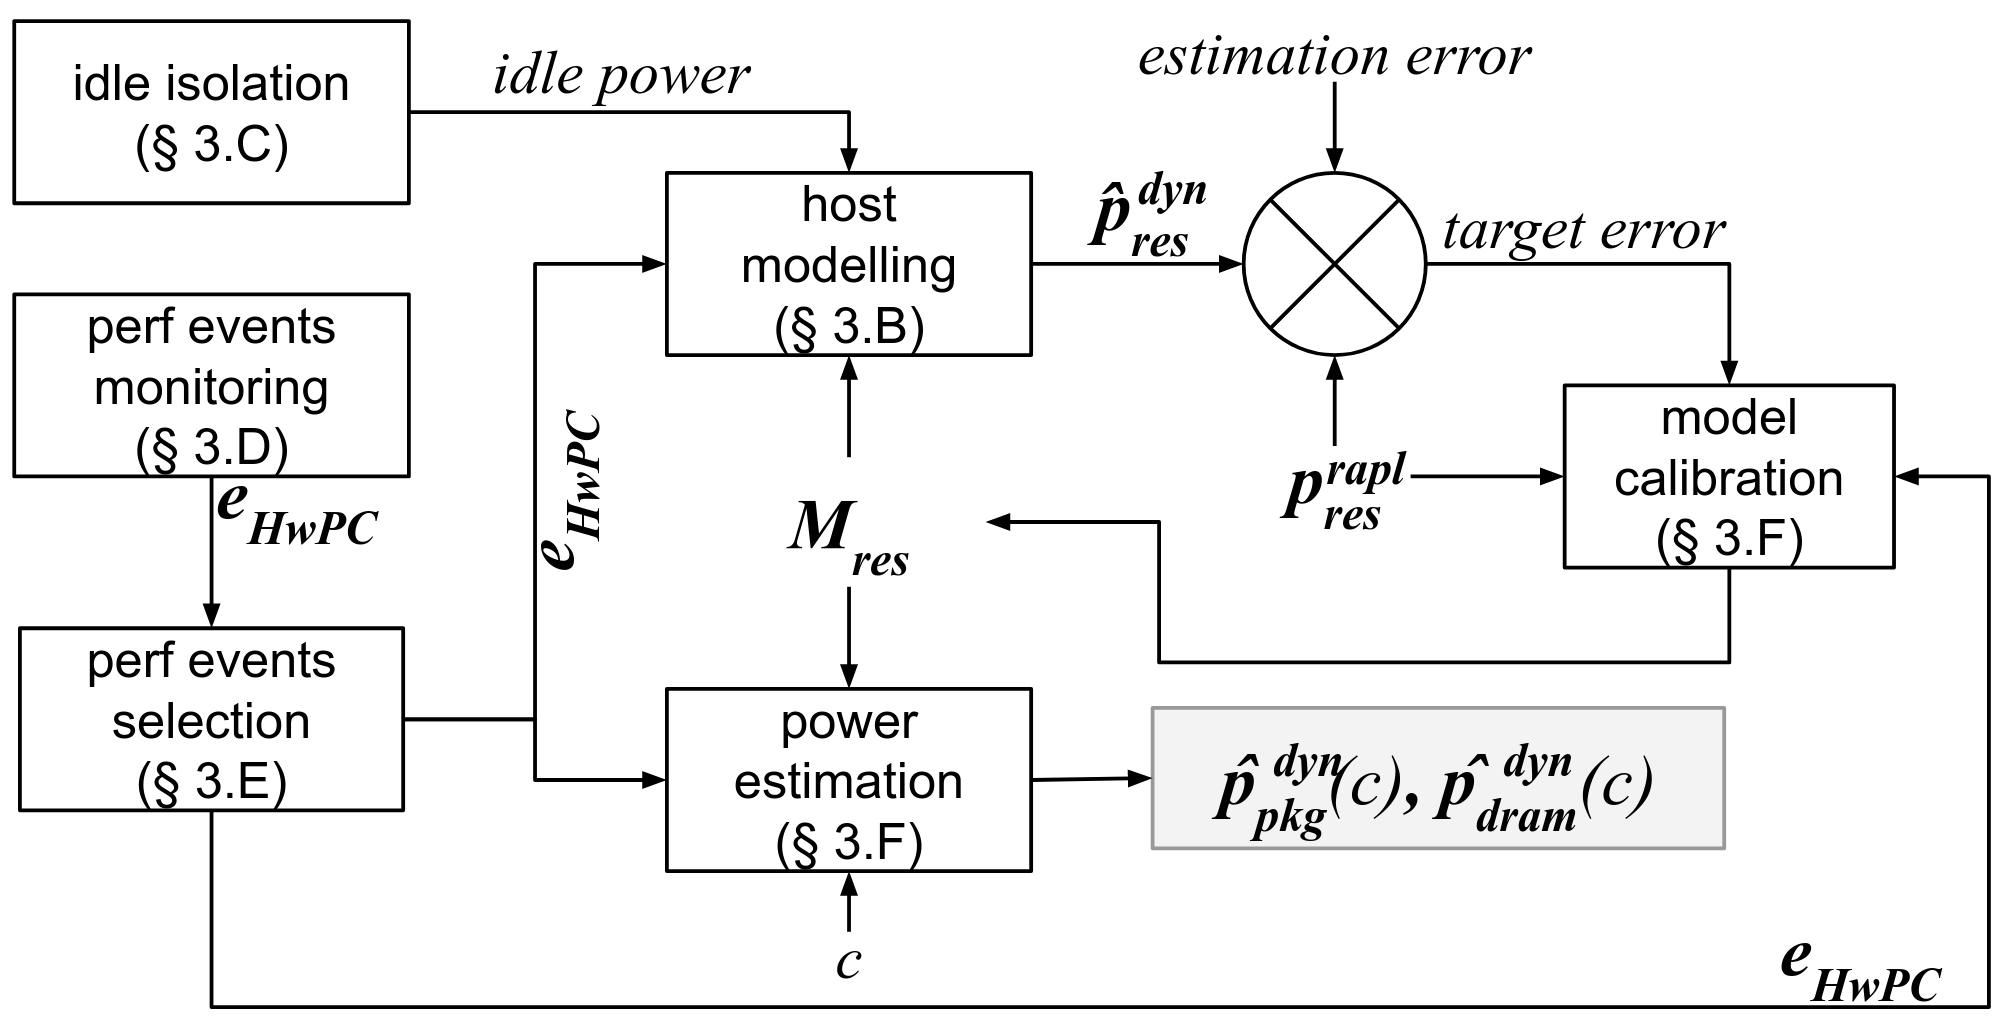
\includegraphics[width=0.7\textwidth]{Figures/smartwatts_architecture.png}
    \caption[SmartWatts architecture]{SmartWatts Architecture}
    \label{fig:smartwatts_architecture}
\end{figure}
\subsubsection{Attribution Model}
\label{sec:smartwatts-attribution}
As discussed in the previous subsection, the SmartWatts attribution model does not use RAPL metrics, opting only for process metrics. SmartWatts separates host energy consumption into static and dynamic power consumption:
\begin{equation}
    p_{res}^{rapl} = p_{res}^{static} + p_{res}^{dynamic}
\end{equation}

\textbf{Static power} is estimated by periodically logging RAPL package and DRAM power consumption. The $median$ value and the $interquartile range$ (IRQ) are gathered from teh measurements to define the static host power consumption as 
\begin{equation}
    p_{res}^{static} := median_{res} - 1.5 \cdot IRQ_{res}
\end{equation}
This approach is meant to filter out RAPL outliers.

\textbf{Dynamic power} is estimated by correlating the CPU frequency $f$ and the raw metrics reported by HWCP:
\begin{equation}
    \exists f \in F, \hat{p}_{res}^{dyn} = M_{res}^{f} \cdot E_{res}^{f}
\end{equation}
where $E_{res}^{f}$ denotes all \textit{events}. The model $M_{res}^{f}$ is build from \textit{elastic net} regression applied on the last $k$ samples. To ensure that all container power consumptions are linear with regards to global power consumption, positive inference coefficients are enforced, and the intercept (or \textit{bias term} is within the range $[0, TDP]$.

\textbf{HWPC metrics} are dynamically chosen based on the list of available events exposed by the host's \textit{Performance Monitoring Units} (PMU), essentially creating a custom model based on available metrics. Not all available metrics are used, and statistical analysis (Pearson coefficient) is used to determining worthy candidates.

\textbf{Container power consumption} is estimated by applying the inferred power model $M_{res}^{f}$ at the scale of the container's events $E_{res}^{f}(c)$, as seen in formula~\ref{for:smartwatts_container_events}. In formula~\ref{for:smartwatts_container_intercept}, the intercept $i$ is distributed proportionally to the dynamic part of the consumption of $c$.
\begin{equation}
\label{for:smartwatts_container_events}
    \exists f \in F, \forall c \in C, \hat{p}_{res}^{dyn}(c) = M_{res}^{f} \cdot E_{res}^{f}(c)
\end{equation}
\begin{equation}
\label{for:smartwatts_container_intercept}
    \forall c \in C, \tilde{p}_{res}^{dyn}(c) = \hat{p}_{res}^{dyn}(c) - i \cdot (1-\frac{\hat{p}_{res}^{dyn}(c) -i}{\hat{p}_{res}^{dyn} -i})
\end{equation}

In theory, one can expect $\hat{p}_{res}^{dyn} \overset{!}{=} {p}_{res}^{dyn}$ if the model perfectly estimates the dynamic power consumption, but in practice, an error $\epsilon_{res} = \left| {p}_{res}^{dyn} - \hat{p}_{res}^{dyn} \right|$. Therefore, container power consumption is capped at
\begin{equation}
    \forall c \in C, \left\lceil \tilde{p}_{res}^{dyn}(c) \right\rceil = \frac{{p}_{res}^{dyn} \cdot \tilde{p}_{res}^{dyn}(c)}{\hat{p}_{res}^{dyn}}
\end{equation}
This approach also allows to calculate a confidence intercal of the power consumption of containers by scaling down the observed global error:
\begin{equation}
    \forall c \in C, \epsilon_{res}(c) = \frac{\tilde{p}_{res}^{dyn}(c)}{\hat{p}_{res}^{dyn}} \cdot \epsilon_{res}
\end{equation}

In order improve estimation accuracy, the following configurable parameters are used:
\begin{itemize}
    \item CPU-TDP in Watt (default: 125)
    \item CPU base clock in MHz (default: 100)
    \item CPU base frequency in MHz (default: 2100)
    \item CPU and DRAM error threshold in Watt (default: 2)
    \item Minimum of samples required before trying to learn a power model (default: 10)
    \item Size of the history window used ot keep samples from (default: 60)
    \item Measurement frequency in milliseconds (default: 1000)
\end{itemize}
\subsubsection{Validation and Research Context}
\label{sec:smartwatts-validation}
With RAPL being used as ground truth for dynamic power estimation model recalibration, it is important to note that the SmartWatts validation is focused on the model accuracy when compared to RAPL values instead of values obtained by an external source of power data. The SmartWatts validation focused on the quality of power estimation in sequential and parallel workloads, the accuracy and sstability of power models and the overhead of the \textit{sensor} component. Standard benchmarks like Stress-NG and NAS parallel Benchmarks were chosen. 

While there is no advanced statistical analysis, the validation shows that, for a error threshold for CPU and DRAM of 5 and 1 Watt respectively, power consumption can be reliably estimated with less than 3 Watts and 0.5 Watts, respectively. The only case where the error grows beyond the threshold is at the CPU idle frequency. The model stability is shown to significantly improve when lower recalibration frequencies are used. SmartWatts succeeds to reuse a give power model for up to 594 estimations, depending on frequency. The monitoring overhead is observed to be at 0.333 Watts for the PKG domain and 0.030 Watts for the DRAM domain on average, at a measurement frequency of 2 Hz. The authors consider this overhead negligable.
\subsubsection{Limitations and Open Issues}
\label{sec:smartwatts-limitations}
SmartWatts offers a compelling solution for dynamic, container-level power estimation through self-calibrating models based on performance counters. However, its applicability remains domain-specific. The central assumption is that RAPL, while accurate, is too coarse-grained for attributing power to individual containers or processes. This premise is debatable: RAPL offers low-overhead, high-frequency measurements, and may be sufficient for many use cases, particularly in homogeneous or single-tenant systems. Whether SmartWatts' added complexity is justified depends on how fine-grained the attribution needs to be.

SmartWatts shines when more granular telemetry (e.g., perf events) is available and container-level attribution is critical. Yet its current implementation models only CPU and DRAM domains, limiting its ability to offer a comprehensive energy profile.

The design allows operators to supply hardware-specific values (e.g. CPU TDP), while falling back to sensible defaults. This improves usability without sacrificing model accuracy.

Finally, while SmartWatts' runtime calibration and dynamic event selection enhance adaptability, they introduce complexity. The event selection mechanism relies on statistical heuristics, which may not generalize well across systems. Moreover, under highly dynamic conditions, frequent recalibrations may affect stability.

In summary, SmartWatts is well-suited for environments requiring high-resolution attribution beyond RAPL's capabilities, but its scope, complexity, and assumptions warrant careful consideration depending on the target use case.


\section{Comparison of Container-Level Tools}
\label{sec:tool-comparison}
\subsection{Feature Comparison}
\label{sec:feature-comparison}
\subsection{Granularity and Metric Sources}
\label{sec:granularity-comparison}
\subsection{Platform Compatibility and Integration}
\label{sec:integration-comparison}

\section{Relevance to Proposed Architecture}
\label{sec:relevance-to-architecture}
\subsection{Lessons Learned from Existing Tools}
\label{sec:lessons-learned}
\subsection{Identified Gaps and Opportunities}
\label{sec:tool-gaps}
\subsection{Implications for Chapter \ref{chap:architecture}}
\label{sec:implications-architecture}

\section{Summary}
\label{sec:tool-summary}




\subsubsection{Overview and Architecture}
% What the tool does, where it runs, general design.
\subsubsection{Metrics and Data Sources}
% What it measures, how it collects (RAPL, perf, eBPF, etc.).
\subsubsection{Attribution Method and Scope}
% How power is assigned to tasks (processes, VMs, containers).
\subsubsection{Validation and Limitations}
% Is it validated? Known weaknesses or constraints?
\subsubsection{Relevance to Proposed Architecture}
% Optional – What ideas or drawbacks will influence your own model.



\begin{comment}
    4.1 Overview of Tool Landscape
        KEPLER, Scaphandre, CodeCarbon, PowerAPI, Cloud Carbon Footprint, etc.
    4.2 Tool Analysis Framework
        Accuracy, data sources, correlation method, platform support, etc.
    4.3 Detailed Evaluation of Selected Tools
        One subchapter per tool:
            4.X KEPLER
            4.X Scaphandr
            ...
    4.4 Comparison Summary
        Table of tradeoffs
        Strengths and weaknesses
        Missing features / open gaps


\section{Tools}
\subsection{RAPL-based tools}
\label{sec:rapltools}
\begin{itemize}
    \item \parencite{jay2023experimental} An experimental comparison of software-based power meters (focus on CPU / GPU)
    \item \parencite{van2025powersensor3} fast accurate opensource: PowerSensor3 enables real-time power measurements of SoC boards and PCIe cards, including GPUs, FPGAs, NICs, SSDs, and domain-specific AI and ML accelerators
    \item \parencite{scaphandre_documentation} Scaphandre. Does not handle overflows correctly (https://github.com/hubblo-org/scaphandre/issues/280)
    \item \parencite{fieni2020smartwatts} Smartwatts: Self-Calibrating Software-Defined Power Meter for containers
    \item \parencite{joularjx} JoularJX: java-based agent for power monitoring at the code level
    \item \parencite{kepler_energy}: KEPLER
    \item \parencite{powertop}: powertop
    \item \parencite{greencodingdocs}: Green metrics tool: measuring energy and CO2 consumption of software through a software life cycle anslysis (SLCA): Metric providers: RAPL, IPMI, PSU, Docker, Temperature, CPU, ... (sone external devices)
    
    % according to raffin2024: simplified versions of scaphandre and codecarbon hhve 3\%, 0.5\% overhead at 10Hz
    % according to \parencite{jay2023experimental}, the full versions have between 2 and 7\% at 1Hz.

    powerAPI            Focuses on per-process measurement, not container nor Kubernetes aware
    WattsUpDoc          Focuses on data center-wide telemetry, not container-level granularity
    Perf/EnergyPerf     Offers per-core/per-task telemetry, but requires extensive integration to map to containers
    PowerTOP            Local profiling tool; not suited for cluster-wide telemetry or Kubernetes
    PowerAPI -> on github contains repos for powerapi, smartwatts-formula, hwpc-sensor, pyjoules
    EnergyVisor
    nvme-cli
    PAPI (uses RAPL)


\parencite{fieni2024powerapi}: PowerAPI: Python framework for building software-defined power
\end{itemize}

- multiple papers have tried to attribute component-level 




\section{Container-Level Monitoring Tools}
    KEPLER, Scaphandre, Smartwatts, JoularJX, AI Power Meter, CodeCarbon.
    Granularity down to the container level.
    internal mechanisms (e.g., eBPF, RAPL, NVML).
    Advantages and drawbacks.
    
\section{Comparison of Tools}
    Detailed matrix comparing:
        Measurement methodology.
        Component focus (CPU, RAM, GPU, Disk, Network).
        Real-time capabilities.
        Kubernetes compatibility.
\end{comment}